\documentclass[letter,12pt]{article}
\usepackage[T1]{fontenc}
\usepackage[tc]{titlepic}
\usepackage[utf8]{inputenc}
\usepackage{lmodern}
\usepackage{amsfonts,amsmath,amssymb}
\usepackage{amsthm}
\usepackage{geometry,listings}
%\geometry{margin=2.5cm}
\usepackage{color,xcolor,moreverb}
\usepackage{tikz,graphicx}
\usepackage{float}
\usepackage{url}
\usepackage{enumitem}
\usepackage[mathcal]{euscript}
\usepackage{tikz,tkz-tab}
\usepackage{genyoungtabtikz}
\usepackage{bbm, bm}
\usepackage{mathrsfs}
\usepackage{xargs}
\usepackage{sagetex}
\usepackage{hyperref}



%Notes
\usepackage[colorinlistoftodos,prependcaption,textsize=small,textwidth=2.5cm]{todonotes}
\newcommand{\pauline}[1]{\todo[linecolor=blue,backgroundcolor=cyan!25,bordercolor=blue]{#1}}
\newcommand{\nicolas}[1]{\todo[linecolor=green,backgroundcolor=green!25,bordercolor=green]{#1}}

% Maths
\newcommand{\RR}{\mathbb{R}}
\newcommand{\KK}{\mathbb{K}}
\newcommand{\NN}{\mathbb{N}}
\newcommand{\ZZ}{\mathbb{Z}}
\newcommand{\QQ}{\mathbb{Q}}
\newcommand{\CC}{\mathbb{C}}
\newcommand{\Sym}[1]{\mathbb{S}_{#1}}
\newcommand{\Elambda}[1]{\mathcal{E}_{#1}}
\newcommand{\Elambdar}[2]{\mathcal{E}_{#1}^{(#2)}}	

\DeclareMathOperator{\Sn}{\mathbb{S}_n}
\DeclareMathOperator{\GLr}{GL_r}
\DeclareMathOperator{\harmonics}{\mathcal{H}}
\DeclareMathOperator{\sgn}{sgn}

\newtheorem{theorem}{Theorem}
\newtheorem{conjecture}{Conjecture}
\newtheorem{prop}{Proposition}
\newtheorem{lemme}{Lemma}
\newtheorem{coroll}{Corollary}
\newtheorem{definition}{Definition}
\newtheorem{example}{Example}


%Tableaux
\newcommand{\diagramme}{\YFrench \Yboxdim{10pt}\yng}
\newcommand{\tableau}{\YFrench \Yboxdim{10pt}\young}
\newcommand{\petitDiagramme}{\YFrench \Yboxdim{5pt}\yng}
\newcommand{\petitTableau}{\tiny \YFrench \Yboxdim{5pt}\young}


%SageTex
\renewcommand{\sagecommandlinetextoutput}{True} % False = output in Latex 
\lstdefinestyle{SageInput}{
	style=DefaultSageInput,
	basicstyle=\small\normalfont\ttfamily,
	numbers=none,
 	breaklines=true, }
\lstdefinestyle{SageOutput}{style=DefaultSageOutput}

%%- 1 ère page
\title{Computing the bicharacter of huge subspaces of polynomials}
\author{Pauline Hubert \and Nicolas Thiéry}



\begin{document}
	
	\maketitle 
	
	\begin{abstract}
		To complete ... 
	\end{abstract}
	
	\tableofcontents

	
	\section{Introduction}
	In this article, we present a new SageMath package to compute bicharacter of some multivariate polynomials spaces. 
	The development of this package started at the occasion of a collaboration with François Bergeron to study the character of the space $\harmonics_n^{(r)}$ of diagonal harmonic polynomials on $r$ sets of $n$ variables, as a graded bi-$\GLr \times \Sn$-module. It is then extended to compute other characters of polynomial spaces. 
	
	The main achievement is a calculation of the character of the diagonal harmonic polynomials for $n=6$ and $r=5$ (and therefore any $r$) in 45 minutes (and ~15Gb), which led to conjectures on its general value.
	
	This is a potentially huge calculation ($\harmonics_6^{(5)}$ is of dimension $5.8 \cdot10^5$), involving polynomials of degree up to $15$ in $30$ variables with thousands of terms. So we have to combine several strategies that each reduced the time and/or memory complexity by one or two orders of magnitude. As much as possible, the code is written to be modular and reusable.

	
	\section{Context : harmonic and diagonal harmonic polynomials}

\nicolas{Ajouter des exemples au fur et à mesure}
\pauline{J'ai déjà mis pas mal d'exemples. Il en faut plus?}
		
	Consider the polynomial ring $R=\QQ[X]$ with $r$ sets of $n$ variables. To fix conventions, we think of $X$ as a matrix of variables:
	$$X := \begin{pmatrix}
	x_{1,1} & x_{1,2} & \cdots & x_{1,n} \\
	x_{2,1} & x_{2,2} & \cdots & x_{2,n} \\
	\vdots & \vdots & \ddots & \vdots \\
	x_{r,1} & x_{r,2} & \cdots & x_{r,n} \\
	\end{pmatrix}$$
	and we denote by $\bm{x}_i = (x_{i,1}, x_{i,2}, \dots, x_{i,n})$ the i-th set of variables. We use the convention that bold letters stand for sets of variables and light letters stand for the variables themselves. 
	
	The polynomial ring $R$ is endowed with an action of the symmetric group $\Sn$ by diagonal permutation of the columns of $X$ and of the general linear group $\GLr$ by diagonal action on the rows of $X$. 
	\begin{figure}[H]
		\centering
		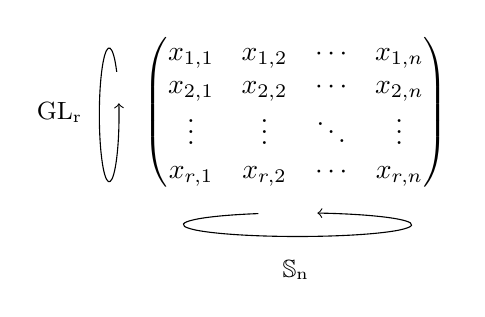
\begin{tikzpicture}
		\draw node{$\begin{pmatrix}
			x_{1,1} & x_{1,2} & \cdots & x_{1,n} \\
			x_{2,1} & x_{2,2} & \cdots & x_{2,n} \\
			\vdots & \vdots & \ddots & \vdots \\
			x_{r,1} & x_{r,2} & \cdots & x_{r,n} \\
			\end{pmatrix}$ } (0,0);
		\draw (-2.4,.3)+(60:.25)
		[xscale=.5,yscale=3.4,->,rotate=80] arc(-40:290:.25);
		\node at (-3,0) {{\small$\GLr$}};
		\draw (-.6,-1.5)+(60:.25)
		[xscale=5.8,yscale=.6,->,rotate=-210] arc(-40:290:.25);
		\node at (0,-2) {{\small$\Sn$}};
		\end{tikzpicture}
		\caption{Simultaneous actions of $\GLr$ and $\Sn$ on $X$.}
	\end{figure}
	
	The invariant ring $R^{\Sn}$ is known as the ring of multisymmetric functions, that is to say the elements of $R$ that remain unchanged under permutations of the rows of $X$. The co-invariant ring $R_{\Sn}$ is the quotient of $R$ by the ideal $\mathcal{I}_n = \langle {R^{\Sn^+}} \rangle$ of the multisymmetric functions without constant term. It inherits from R a structure of graded $\GLr \times \Sn$ bi-module. The degree of a polynomial in $R_{\Sn}$ is defined to be the sum of the degrees in each set of variables. 
	
	The natural grading of $R$ can be refined into a multigrading by rows. The multigrading is preserved by the action of $\Sn$. The multigrading is not preserved by the action of $\GLr$, but instead carries exactly the information about the $\GLr$-character. It is thus equivalent to consider the $\GLr \times \Sn$-bicharacter or the $\Sn$ multigraded character of $R_{\Sn}$. \\
	
	
	We denote the partial derivatives by $\partial^k_x := \frac{\partial^k}{\partial x^k}$ for all variables $x \in X$.
	When $X$ contains only one set of variables, $X = (x_1, x_2, \dots, x_n)$, we define the \emph{harmonic polynomials} as follow.
	
	\begin{definition}
		Let $f \in R$, $f$ is \emph{harmonic} if and only if, for all $k \geq 0$,
		$$\partial^k_{x_1} f + \partial^k_{x_2} f + \dots + \partial^k_{x_n} f = 0.$$
	\end{definition}

	The space of harmonic polynomials in $n$ variables, denoted $\harmonics_{n}$, is the joint kernel of the differential operators $D_k := \partial_{x_1}^k + \cdots + \partial_{x_n}^k$. It is also a realization of the coinvariants of the symmetric group: $R\, /\, \langle Sym(X)^+ \rangle$ and a graded regular representation of $\Sn$. 
	
	\begin{example}
		The Vandermonde determinant $V_n:= \det(x_i^a)_{1 \leq i \leq n \atop 0 \leq a \leq n-1} = \prod_{i<j}(x_i-x_j)$ is harmonic.
		
		The space of harmonic polynomials in two variables is $\harmonics_2 = \langle 1, x_1-x_2 \rangle_\QQ$. 
	\end{example}
		
	It is easy to see that if $f$ is harmonic then $\partial_{x_i} f$ is also harmonic for all $x_i \in X$. Using that, one can define $\harmonics_{n}$ directly with  partial derivatives instead of seeing them as solutions of a system of partial differential equations as stated in the following theorem. See \cite{Haiman2002} and \cite{Bergeron2009} for more details. 
	
	\begin{theorem}
		The space of harmonic polynomials $\harmonics_{n}$ is the smallest subspace containing the Vandermonde determinant $V_n$ and closed by partial derivatives.
	\end{theorem}
	
	Going back to an arbitrary number $r$ of sets of variables, we define the \emph{differential operators} $(D_\alpha)_{\alpha\in \NN^r}$:
	$$D_{(\alpha_1, \dots, \alpha_r)} := \partial_{x_{1,1}}^{\alpha_1}\dots\partial_{x_{r,1}}^{\alpha_r} + \dots + \partial_{x_{1,n}}^{\alpha_1}\dots\partial_{x_{r,n}}^{\alpha_r}$$
	
	\begin{example}
		Take $r=3$ and denote $\bm{x}, \bm{y}$ and $\bm{z}$ the three sets of variables of $X$, then $D_{(3,0,4)} := \partial_{x_1}^3\partial_{z_1}^4 + \dots + \partial_{x_n}^3\partial_{z_n}^4$. 
	\end{example}

	\begin{definition}
		The space of \emph{diagonal harmonic polynomials} $\harmonics_n^{(r)}$ is the joint kernel of the differential operators $(D_\alpha)_\alpha$. Note that $\harmonics_n^{(r)}$ contains $\harmonics_{n}^{(1)} = \harmonics_{n}$.
	\end{definition}
	
	As for harmonic polynomials, we have an alternative way to obtain $\harmonics_n^{(r)}$ directly using operators. 
	
	\begin{definition}
		The \emph{polarisation operator} $P_{x,y}^k$ is given by
		$$P_{x,y}^k = \sum_{i=1}^{n} y_i \partial_{x_i}^k$$
		where $\bm{x}$ and $\bm{y}$ are two sets of variables of $X$. 
	\end{definition}
	
	For $k=1$, those operators implement the action of $\mathfrak{sl}_r$ induced by $\mathfrak{gl}_r$.
	
	\begin{theorem} \pauline{Nicolas as-tu la réf pour ce thm?}
		Multisymmetric polynomials are obtained by polarization of symmetric polynomials in the first set of variables.
	\end{theorem}
	
	\begin{conjecture} \label{DiagHarm}
		Diagonal harmonic polynomials $\harmonics_n^{(r)}$ are obtained by polarization of harmonic polynomials $\harmonics_n^{(1)}$ in the first set of variables.
	\end{conjecture}
	
	Conjecture \ref{DiagHarm} has been proven for two sets of variables (see for example \cite{Bergeron2009}). It is not proven yet for more than two sets of variables but it has been verified by computation by Mike Zabrocki for a large number of sets of variables so we assume it to be true. \pauline{talk to Mike for more informations} \\

     
    Since diagonal harmonics polynomials spaces are of huge dimension, they are not easy to study. Indeed, when $r=1$, $R_{\Sn}$ is of dimension $n!$, and when $r=2$, $R_{\Sn}$ is of dimension $(n+1)^{n-1}$ ($16807$ for $n=6$).
    
    In order to study those spaces, we use representation theory and characters.  Intuitively, we want to decompose modules into irreducible submodules according to the group action. Those submodules are then represented by irreducible characters that encode the group action on each submodule. For $\GLr$ and $\Sn$, irreducible characters can be indexed by partitions and encoded by Schur functions. Knowing the irreducible characters gives information on the studied module such as the dimension. 
    
    We don't enter into details on representation theory here but for more on this topic see \cite{FultonHarris1991}. Also, \cite{Sagan} is a classical reference for representation theory of the symmetric group and \cite{Green2007} is about polynomial representations of the general linear group. \\ 
   	
   	
   	The characters of the harmonic and diagonal harmonic polynomial spaces have been studied a lot until now. For example, it is known that, when r=1, the action of $GL_1$ is trivial and $R_{\Sn}$ carries the usual graded representation of $\Sn$. Its character is given by a Hall-Littlewood polynomial.
   	
    The case r=2 has been studied by Garsia and Haiman (see \cite{GarsiaHaiman1993}) and the bigraded character, as a consequence of Haiman's proof of the $n!$-conjecture (see \cite{Haiman2002}), is a Macdonald polynomial.
    
	Finally, some progress in the case $r=3$ had recently been made by Bergeron and Préville-Ratelle (see \cite{BergeronPreville2012}), but the general case is still unknown. Therefore, the computation of the characters of $\harmonics_{n}^{(r)}$ should lead to a better understanding of those spaces. \\
	
	Throughout this article, we write the spaces and their the character the same way, except if there might be a confusion, then the variables are added to the character and we write $\mathcal{H}_n^{(r)}(\bm{q};\bm{w})$ for the character of $\mathcal{H}_n^{(r)}$,  with $\bm{q}$ the variables used to express the $\GLr$ part of the character and $\bm{w}$ for the $\Sn$ part.\\
	
	In the next section, we expose strategies used to go further in the computation of those characters. Those strategies are not limited to the diagonal harmonic polynomials. They can be used in other generalizations. We introduced some of these generalizations in the last section and discuss some applications of these computations.
	 
	
	\section{Strategies}
	
	\subsection{Computing in the space of harmonic polynomials using polarization}
	
	We first need to compute in a quotient by an ideal, $R / \mathcal{J}_n$ where $\mathcal{J}_n = \langle Sym(X)^+ \rangle$ is the ideal of diagonal symmetric polynomials on $r$ sets of $n$ variables.
	A standard approach would be to compute a Gröbner basis of this ideal.
	We haven't actually tried it, but given the number of variables and dimension of the quotient, we expect this calculation to be intractable.
	
	So we take the classical route of realizing the coinvariant ring as the space $\harmonics_n^{(r)}$ of diagonal harmonic polynomials.
	This is the space of those polynomials that satisfy the equations given by the multisymmetric functions seen as differential operators.
	
	Solving those differential equations would not be tractable either. So instead we use partial derivatives and polarization operators defined in the previous section. \\
	
	In practice, we implemented a general purpose utility in Sage, \texttt{Subspace(vectors, operators)} that computes the smallest subspace of a vector space which contains the given vectors and is stable under the action of the given linear operators.
	
	\begin{example} \label{H_3} Compute $\harmonics_3$ with one row of variables $\bm{x} = (x_1, x_2, x_3)$. \pauline{I haven't find yet a way to have latex output with automatic breaklines.}
		\begin{sagesilent}
			load("../subspace.py")
		\end{sagesilent}
		\begin{sagecommandline}
			sage: R = QQ['x1,x2,x3']
			sage: M = matrix.vandermonde(R.gens(), R)
			sage: M
			sage: derivatives = [attrcall('derivative', x) for x in R.gens()]
			sage: H_3 = Subspace([M.determinant()], derivatives)
			sage: H_3.basis()
			sage: H_3.dimension()
		\end{sagecommandline}	
	\end{example}
	
	We simply do linear algebra here. We maintain a matrix in row echelon form representing a basis of the space computed so far, and a ToDo list of $op(v)$, that remain to be computed and inserted in the matrix, where $op$ is an operator and $v$ an element of the subspace in construction.
	
	This utility should already have been in Sage, and will end up there. \\
	
	Once a basis of $\harmonics_n^{(r)}$ is constructed, there still remains to recover its bicharacter. For $\GLr$ that's given by the multigrading. For $\Sn$ some additional work has to be done (e.g. computing the traces of the action of permutations of all cycle types).
	
	At this stage, we have an algorithm, but are still doing linear algebra in a huge space. The cost is $N^2 M$, where $N$ is the dimension of the result and $M$ the dimension of the ambient space.
	
	\subsection{Exploiting the multigrading}
	
	The \texttt{Subspace} utility can be adapted to exploit the multigrading. The input is now a collection of homogeneous vectors and operators together with their multidegrees, and a separate row echelon matrix is maintained for each multidegree.
	
	\begin{example} Compute $\harmonics_{3}^{(2)}$ using the multidegree. 
		\begin{sagesilent}
			load("../character.py")
		\end{sagesilent}
		First, we compute $\harmonics_{3}^{(1)}$, for one row of variables. 
		\begin{sagecommandline}
			sage: v = vandermonde(3)
			sage: v
			sage: derivatives = partial_derivatives(v.parent())
			sage: derivatives
			sage: H_3 = Subspace({v.multidegree(): [v]}, derivatives)
			sage: H_3.basis()
			sage: H_3.dimension()
		\end{sagecommandline}
		Then, we use polarization operators to introduce a second set of variables, and thus obtain $\harmonics_3^{(2)}$, still with multidegree. 
		\begin{sagecommandline}
			sage: polarizators = polarization_operators(2)
			sage: polarizators
			sage: H_3 = PolarizedSpace(H_3, polarizators)
			%sage: H_3.basis()
			sage: H_3.dimension()
			sage: H_3.dimensions()
		\end{sagecommandline}
		Compared with example \ref{H_3} in which all basis elements are grouped in one list with key $0$, here basis elements are classified by multidegree with the corresponding key. Operators are also separated by multidegree. Moreover, we have access to dimension by multidegree. 
	\end{example}
	
	Note that \texttt{PolarizedSpace} takes in argument a \texttt{Subspace} from which it extracts the basis and returns a \texttt{Subspace} build from this basis and the given operators. The difference is that, this time, the computation is adapted to take care of the change of polynomial ring between one and two (or more) sets of variables. \\
	
	There are two advantages of considering the multidegree. 
	First, writing $N=:\sum N_D$, the complexity becomes $(\sum N_D^2) M$ instead of $(\sum N_D)^2M_D$ (in fact better).
	Second, the multidegrees, and therefore $\GLr$ character, can be directly read off the result.
	
	\subsection{Exploiting representations of the symmetric group}
	
	The $\GLr$-character can easily be recover from the multigrading, but it remains to find an efficient way to compute the representations of $\Sn$. Computing the traces of the action of permutations of all cycle types would not be an option because of the dimension and the high number of terms of the polynomials. 
	Instead, we use an isotypic projector to obtain the isotypic components of $\Sn$ and from that we will be able to recover the irreducible characters of $\Sn$ with their multiplicities. \\
	
	We first define two elements of the symmetric group algebra $\CC \Sn$. Note that we use the cyclic notation for permutations.
	Let $P_{\mu}$ be the subgroup of $\Sn$ of all row preserving permutations of $\mu$ and $Q_{\mu}$ the subgroup of all column preserving permutations of $\mu$. 
	
	To determine the row and column preserving permutations, we consider the canonical Young tableau of $\mu$, that is to say the tableau filled in by integers from $1$ to $n$ in increasing order, from left to right and from bottom to top. Then a permutation is said row (resp. column) preserving if when applied to the canonical tableau of $\mu$, the entries of each row (resp. column) remains in the same row (resp. column) maybe in a different order (see example \ref{young_idempotent}).  
	
	With those subgroups, we define $a_{\mu} = \sum_{\sigma \in P_{\mu}} \sigma$ and  $b_{\mu} = \sum_{\sigma \in P_{\mu}} \sgn(\sigma) \sigma$. And finally, the \emph{Young symmetrizer} is the element $$c_{\mu} = a_{\mu} b_{\mu}.$$
	
	The Young symmetrizer is also called \emph{Young idempotent}. See \cite{FultonHarris1991} for more on this. 
	
	\begin{example}\label{young_idempotent} Let $\mu = (2,1)$.
		The canonical tableau associated is \tableau(12,3).
		
		Then $P_\lambda = \{1, (12)\}$ and $Q_\lambda = \{1, (13)\}$. 
		 
		For $\mu=(2,1)$, we have
		$a_{2,1} = 1 + (12)$ and
		$b_{2,1} = 1 - (13)$. 
		
		Therefore, $c_{2,1} = (1 + (12)) . (1 - (13)) = 1 + (12) - (13) - (132)$. 
		
		For the other partitions of size $3$, one can verify that 
		$c_{1,1,1} = \sum_{\sigma \in \Sym{3}} \sigma$ and 
		$c_{3} = \sum_{\sigma \in \Sym{3}} \sgn(\sigma)\sigma$.
	\end{example}
	
	\begin{theorem}
		The Young symmetrizer $c_{\mu}$ is idempotent up to a scalar and the image of $c_{\lambda}$ by right multiplication on $\CC \Sn$ is an irreducible representation $A_{\mu}$ of $\Sn$.
		Thus any irreducible representation can be obtain this way for a unique partition. 
	\end{theorem}
	
	The proof of the above theorem is given by Fulton and Harris in \cite{FultonHarris1991}. 
	This theorem guarantees that $c_{\mu}$ is an isotypic projector. Thus applying $c_\mu$ on $\harmonics_{n}^{(r)}$ gives the $\Sn$-isotypic component of type $\mu$ of $\harmonics_{n}^{(r)}$. Moreover, using an adapted basis \pauline{On a vraiment besoin d'une base particulière?} of $\harmonics_{n}^{(r)}$ guarantees that we obtain enough elements to be able to construct a basis of the isotypic component and thus we obtain the multiplicity of the irreducible representation of $\Sn$ corresponding to $\mu$. \\
	
	The action of $\GLr$ commutes with the action of $\Sn$, then the polarization operators commute with the Young symmetrizer. Therefore, in practice, we can compute independently each $\Sn$ isotypic component of $\harmonics_{n}^{(r)}$ by starting from a basis of $\harmonics_{n}^{(1)}$ and decomposing it into isotypic components:
	$$\harmonics_{n}^{(1)}:=\bigoplus_{\mu \vdash n} \harmonics_{\mu}^{(1)},$$
	
	where $\harmonics_{\mu}^{(1)}$ is the isotypic component of type $\mu$ of $\harmonics_{n}^{(1)}$.
	
	Then we use the polarization operators to obtain all the isotypic components $\harmonics_{\mu}^{(r)}$ of $\harmonics_n^{(r)}$ ($r>1$) from those of $\harmonics_n^{(1)}$ .
	
	\begin{example} \label{multigrading}
		Compute $\harmonics_3^{(2)}$ using the Vandermonde determinant for $n=3$. We still use the multigrading. 
		\begin{sagecommandline}
			sage: v = vandermonde(3)
			sage: derivatives = partial_derivatives(v.parent())
			sage: H_3 = Subspace({v.multidegree(): [v]}, derivatives)
		\end{sagecommandline}
		At this stage, we project onto the isotypic components of $\Sym{3}$.
		\begin{sagecommandline}
			sage: H_3 = IsotypicComponent(H_3, 3)
			sage: H_3
		\end{sagecommandline}
		The result is now a dictionnary of subspaces, one for each isotypic component.
		\begin{sagecommandline}
			sage: H_3[Partition([3])].basis()
			sage: H_3[Partition([2,1])].basis()
			sage: H_3[Partition([1,1,1])].basis()
		\end{sagecommandline}
		We polarize each isotypic component. Note that, \texttt{PolarizedSpace} can receive a dictionary of subspaces, each subspace is then considered separately. 
		\begin{sagecommandline}
			sage: H_3 = PolarizedSpace(H_3, polarization_operators(2))
			sage: H_3[Partition([2,1])].basis()
		\end{sagecommandline}
	We print only the polarized isotypic component of type $(2,1)$ to avoid unreadable outputs in this example. 	
	\end{example}
		
	In fact we can do better. \pauline{Does it work only for $\harmonics_n^{(r)}$ or also for $\Elambda{\lambda}$?}
	Fix a partition $\mu$. Recall that a basis of the Specht module $S_\mu$  is given by the family of Garnir/Specht polynomials $(G_{P})_P$ indexed by standard tableaux $P$ of shape $\mu$.
	
	To get a basis of the full isotypic component $\harmonics_{\mu}$ of $\harmonics_n$, we can, for example, use a generalization of this construction (see \cite{Ariki1997}): a family of polynomials $(G_{P,Q})_{P,Q}$ indexed by a pairs $(P,Q)$ of standard tableaux of shape $\mu$ where $Q$ specifies the copy of $S_\mu$ and $P$ specifies the location within that copy of $S_\mu$.
	
	
	For a fixed tableau $P$, denote by $\harmonics_P^{(r)}$ the space spanned by the higher Specht polynomials $(G_{P,Q})_Q$ under polarization. It's exactly the image of $\harmonics_n$ under the Young idempotent associated to $P$. For a given shape $\mu$, the $\harmonics_P^{(r)}$ are all conjugate under $\Sn$, and their direct sum is the isotypic component $\harmonics_{\mu}^{(r)}$.
	
	To conclude, it is sufficient to compute $\harmonics_P^{(r)}$ for one tableau of each shape $\mu$. This reduces the complexity by the square of the number of standard tableaux of shape $\mu$.
	
	However, for now we have not managed to fully implement this strategy but are still working on it. 
	
	\subsection{Exploiting column antisymmetries}
	
	One thing that can slow down the computation is that the polynomials we are working with tend to be big. For example, for $\lambda \vdash 6$, the Vandermonde determinant $V_\lambda$, is a homogeneous polynomial of degree $\sum_{i=1}^{5}i = 15$ with $6!=720$ monomials . This means that we need a lot of space to store them and it takes time when we want to apply operators. 
	
	However, since we use the Young symmetrizer to construct $\harmonics_{n}^{(r)}$, for all $v \in \harmonics_{n}^{(r)}$, $v$ is anti-symmetric with respect to the column stabilizer $Q_\mu$, with $\mu$ the type of the isotypic component of $v$. Indeed, when projecting a polynomial $p$ on its isotypic component using the Young idempotent $c_\mu$, by definition $p.a_\mu$ is symmetric with respect to the row preserving permutations of $\mu$ and then $v = p.a_\mu.b_\mu$ is anti-symmetric with respect to the column preserving permutations of $\mu$. 
	It is therefore sufficient to keep one representative monomial per $S_P$ orbit \pauline{$S_P$ orbit?} (and do some appropriate straightening whenever a new monomial is created). We chose to keep the smallest representative monomial in lexicographic order and call the result the \emph{normal reduced form} of $v$. \\
	
	Thus keeping reduced forms of the polynomials decreases space complexity, and also time complexity when applying operators. Note that each time a polarization operator is applied to an element, the normal reduced form of the new element obtained is computed again. 
	
	\begin{example} ~
		
		$V_{3} = -x_{1}^{2} x_{2} + x_{1} x_{2}^{2} + x_{1}^{2} x_{3} - x_{2}^{2} x_{3} - x_{1} x_{3}^{2} + x_{2} x_{3}^{2}$ is of type $(1,1,1)$ and has reduced form $x_1^2x_2$.
		
		$\partial_{x_2}V_{3} = -x_{1}^{2} + 2 x_{1} x_{2} - 2 x_{2} x_{3} + x_{3}^{2}$ is of type $(2,1)$ and has reduced form $x_1^2 - 2x_1x_2$.
	\end{example}

	In practice, the antisymmetries are exploited first when projecting $\harmonics_n^{(1)}$ onto its isotypic components. When applying the Young idempotent, the reduced form of each element is computed. From this step, the polynomials lie in a diagonal polynomial ring with antisymmetries, thus each polynomial carries the information of its antisymmetries.  
	Then, we maintain the elements of the bases of the isotypic components in their reduced form during polarization. 

	\begin{example}
			Compute $\harmonics_3^{(2)}$ exploiting antisymmetries. 
		\begin{sagecommandline}
			sage: v = vandermonde(Partition([3]))
			sage: derivatives = partial_derivatives(v.parent())
			sage: H_3 = Subspace({v.multidegree(): [v]}, derivatives)
		\end{sagecommandline}
		At this stage, we project onto the isotypic components of $\Sym{3}$ exploiting antisymmetries. One can check the difference between this computation and the one in example \ref{multigrading}. 
		\begin{sagecommandline}
			sage: H_3 = IsotypicComponent(H_3, 3, use_antisymmetry=True)
			%sage: H_3[Partition([3])].basis()
			sage: H_3[Partition([2,1])].basis()
			sage: H_3[Partition([1,1,1])].basis()
		\end{sagecommandline}
		We see that the parent of the polynomials carries the information about the antisymmetries to keep polynomials in normal reduced form.
		\begin{sagecommandline}
			sage: p = H_3[Partition([2,1])].basis().values()[0][0]
			sage: p
			sage: p.parent()
		\end{sagecommandline}
		Now we polarize each isotypic component still exploiting antisymmetries.  
		\begin{sagecommandline}
			sage: H_3 = PolarizedSpace(H_3, polarization_operators(2))
			sage: H_3[Partition([2,1])].basis()
		\end{sagecommandline}
	\end{example}
	
	This trick was already used by François Bergeron for the polarizations of the Vandermonde (the diagram space). Using higher Specht polynomials further allowed  to generalize that optimization to each shape.
	
	We gain in theory up to $n!$. In practice, between one and two orders of magnitude due to the overhead of straightening monomials.
	
	\subsection{Exploiting row symmetries}
	
	The space $\harmonics_{n}^{(r)}$ is symmetric with respect to permutation of rows of $X$, and such permutations exchange multigraded components. For example, for $r=3$, the homogeneous components of respective multidegree $(4,2,1)$ and $(2,1,4)$ coincide up to cycling of the rows. This means that there are polynomials in different homogeneous components that are the same up to a permutation of the sets of variables and that we have redundant information. 
	
	It is therefore sufficient, in principle, to compute homogeneous components with decreasing multidegree. Thus, we reduce memory complexity since not every homogeneous components are kept in memory and time complexity by decreasing the number of polynomials on which apply operators. 
	
	To achieve this, polarization operators can be tweaked. Whenever the result of a polarization is not of decreasing multidegree, straighten it by applying an appropriate permutation of the rows. It can then easily be shown that those tweaked polarization operators properly generate the whole $\harmonics_{n}^{(r)}$ space from $\harmonics_n^ {(1)}$. \pauline{Tweaked polarizators don't generate the whole space only the decreasing multidegree components, right?}
	
	\begin{example} ~ 
		
		The polynomial $x_1^2 - 2x_1x_2 + 2x_2x_3 - x_3^2 \in \mathcal{H}_{3}^{(2)}$ has multidegree $(1,0)$ so the same polynomial with multidegree $(0,1)$ that is $y_1^2 - 2y_1y_2 + 2y_2y_3 - y_3^2$ also appears in $\mathcal{H}_{3}^{(2)}$ but it is not necessary to compute it explicitly.  
		%$-2x_{1} y_{1} y_{2} + x_{1} y_{2}^{2} \in \mathcal{H}_{3}$ so $-2y_{1} x_{1} x_{2} + y_{1} x_{2}^{2} \in \mathcal{H}_{3}$
	\end{example}

	In practice, when we polarize $\harmonics_{n}^{(1)}$, tweaked polarization operators are given in argument to \texttt{PolarizedSpace} instead of the classical ones. As said above, when specifying the row symmetries, only components of decreasing multidegree appear in the final result. 
	
	\begin{example} Exploiting both antisymmetries of columns and row symmetries, the homogeneous components for $\harmonics_3^{(2)}$ become the following.
		\begin{sagesilent}
			v = vandermonde(Partition([3]))
			derivatives = partial_derivatives(v.parent())
			H_3 = Subspace({v.multidegree(): [v]}, derivatives)
		\end{sagesilent}
		\begin{sagecommandline}
			sage: H_3 = IsotypicComponent(H_3, 3, use_antisymmetry=True)
			sage: H_3 = PolarizedSpace(H_3, polarization_operators(2, row_symmetry="permutation"))
			sage: H_3[Partition([1,1,1])].basis()
			sage: H_3[Partition([2,1])].basis()
			sage: H_3[Partition([3])].basis()
		\end{sagecommandline}	
	We observe that only decreasing multidegree components still appear, we don't have components of multidegree $(1,2)$, $(0,3)$, $(0,2)$ and $(0,1)$.
	\end{example}
	
	By exploiting this symmetries, we gain an order of magnitude.\\
	
	As said before, the $\GLr$-character of $\harmonics_n^{(r)}$ is given by the multidegree of the homogeneous components. In other words, for a given isotypic component $\harmonics_{\mu}^{(r)}$, $\mu \vdash n$, the $\GLr$-character associated to this component is given by $$\sum_{\harmonics_{\mu,d}^{(r)}} q^{d}$$ where the sum is over all homogeneous component $\harmonics_{\mu,d}^{(r)}$ of type $\mu$ and multidegree $d$ and $q^d = q_1^{d_1}q_2^{d_2}\dots$.
	
	When exploiting the row symmetries, since we compute only the homogeneous components of decreasing multidegree, we can not compute the character of $\GLr$ using such a summation. However, we know that if we have a component of multidegree $d=(d_1, d_2, \dots, d_k)$ , this correspond to a term $\sum_{\sigma \in \Sym{k}} q^{\sigma(d)} = m_d$ in the previous sum, thus we use monomials symmetric functions $m_d$ instead of summations to recover the character of $\GLr$ in each isotypic component.
	\pauline{Add time computation comparison (with and without optimisations) ?} \\
	
	For now we don't avoid compute some unnecessary homogeneous component since all we do is straighten the polynomials if they don't have decreasing multidegree. It would be even better if we could avoid completely the computation of those polynomials. It is not possible for now because we don't know yet which operators should not been applied to avoid those polynomials. \\
	
	Finding an efficient way to generate $\harmonics_{n}^{(r)}$ is the main part of the computation. Once we have the isotypic components separated by multidegree, we obtain immediatly the character. 
	
	\begin{example} We compute the character of $\harmonics_{3}^{(r)}$. Since we exploit row symmetry, we have to specify it in order to use monomials instead of sums as explain above. 
		\begin{sagecommandline}
			sage: character(H_3, row_symmetry="permutation")
		\end{sagecommandline}
	We finally obtain that the character of $\harmonics_{3}^{(r)}$ for $r \geq 2$ is $$\harmonics_{3}^{(r)} = 1 \otimes s_{3} +(s_{1} + s_{2}) \otimes s_{2,1} +(s_{1,1} + s_{3}) \otimes s_{1,1,1}.$$
	\end{example}
	
	\subsection{Exploiting representations of $sl_k$}
	
	\pauline{I changed nothing in the two following subsections. I leave it to you Nicolas.}
	Building on the previous strategy, it would be tempting to only compute the subspace of $sl_r$ highest weight vectors within each $\harmonics_k^P$.
	
	The current code partially achieves this by avoiding the use of polarization operators of degree $0$ (which clearly would leave the space of highest weight vectors). The obtained space is still too big, and the actual highest weight vectors are obtained by computing the anihilator of the polarization operators $P_{i,i-1}^1$.
	
	The first step requires an additional, not yet proven, trick.
	
	We are currently exploring how to tweak the polarization operators to stabilize the space of highest weight vectors.
	
	\textbf{Current gain:} another order of magnitude; down from 3 days to 45 minutes for $\harmonics_{6;1^6}^{(5)}$
	
	\textbf{Potential gain:} another order of magnitude, both in time and memory.
	
	\subsection{Exploiting the skew commutation of polarization operators}
	
	The polarization operators skew commute. Therefore it would be in principle sufficient to apply them in some "decreasing order". This sounds promising given that, at this stage about 90\% of the polynomials that are produced are redundant and reduced to zero by the linear algebra.
	
	However we have not yet been able put to use that optimization together with the other $sl_k$ optimizations, because the tweaked polarization operators don't skew commute consistently.
	
	\section{Applications / Generalizations}
	
	\subsection{Inert variables} \label{section_inert_variables}
	\nicolas{2-3 paragraphs of announcement in the introduction}
	In their article \cite{GarsiaHaiman1993}, Garsia and Haiman introduce a generalized version of the Vandermonde determinant and a generalization of the diagonal harmonics for two sets of variables called the Gasia-Haiman modules. 
	
	Let $\bm{x}=(x_1, x_2, \dots, x_n)$ and $\bm{y}=(y_1, y_2, \dots, y_n)$ be two sets of variables and $\lambda$ be a partition of $n$. We also denote $\lambda$ the Ferrer's diagram (in French notation) associated to the partition $\lambda$ and each cell of $\lambda$ is given by the Cartesian coordinates $(a,b)$ of its bottom left corner. Then, let define
	$$M_{\lambda} := \det (x_i^ ay_i^ b)_{1 \leq i \leq n \atop (a,b) \in \lambda}$$
	and the Gasia-Haiman module associated to $\lambda$ is the smallest subspace containing $M_{\lambda}$ and closed under differentiation for both sets of variables. \\
	
	With a similar idea, François Bergeron introduce another generalization of the diagonal harmonics, with \emph{inert variables}. We add a new row $\bm{\theta} = (\theta_1, \theta_2, \dots, \theta_n)$ of variables in $X$ and call them inert. The symmetric group still acts by permutation of the columns of $X$, but $GL_r$ now acts diagonally only on the $r$ rows containing non-inert variables.
	
	Note that inert variables, like constants, do not contribute to the degree of the polynomials in which they intervene. They can be considered as "degree 0 variables".  
	
	\begin{figure}[H]
		\centering
		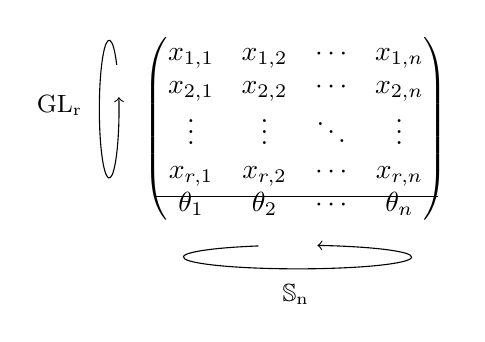
\begin{tikzpicture}
		\draw node{$\begin{pmatrix}
			x_{1,1} & x_{1,2} & \cdots & x_{1,n} \\
			x_{2,1} & x_{2,2} & \cdots & x_{2,n} \\
			\vdots & \vdots & \ddots & \vdots \\
			x_{r,1} & x_{r,2} & \cdots & x_{r,n} \\ 
			\theta_{1} & \theta_{2} & \cdots & \theta_{n}
			\end{pmatrix}$ } (0,0);
		\draw (-2.4,.6)+(60:.25)
		[xscale=.5,yscale=3.5,->,rotate=80] arc(-40:290:.25);
		\node at (-3,0.3) {{\small$\GLr$}};
		\draw (-.6,-1.7)+(60:.25)
		[xscale=5.8,yscale=.6,->,rotate=-210] arc(-40:290:.25);
		\node at (0,-2.1) {{\small$\Sn$}};
		\draw (-1.8,-.85) -- (1.8,-.85);
		\end{tikzpicture}
		\caption{Simultaneous actions of $\GLr$ and $\Sn$ on classical and inert variables.}
	\end{figure}
	
	Let $\lambda$ be a partition of $n$ and note $(a,b)$ the Cartesian coordinates of its cells. Then the determinant $V_{\lambda}$ associated to $\lambda$ is given by $$V_{\lambda} := \det (x_i^a \theta_i^b)_{1 \leq i \leq n \atop (a,b) \in \lambda} .$$
	
	\begin{example}
		The partition $(2,1)$ contains the cells $(0,0)$ and $(1,0)$ in the first row, and the cell $(0,1)$ in the second row, and $V_{2,1} = -x_2\theta_1 + x_3\theta_1 + x_1\theta_2 - x_3\theta_2 - x_1\theta_3 + x_2\theta_3$. 
	\end{example}
	
	
	Like before, we consider the smallest subspace containing $V_{\lambda}$ and closed by partial derivation and polarization, except that this time the inert variables do not intervene in these operators. We denote this space by $\Elambdar{\lambda}{r}$. The space of diagonal harmonics $\harmonics_n^{(r)}$ is thus a special case of $\Elambdar{\lambda}{r}$ for $\lambda = (n)$. \\
	
	The character of $\Elambdar{\lambda}{r}$ stabilizes for $r \geq n$ (see \cite{Bergeron2013} or \cite{Bergeron2009}). Therefore, when the precision is not necessary, we drop the exponent and simply write $\Elambda{\lambda}$ for $\Elambdar{\lambda}{r}$ with $r \geq n$. 
	
	This property also gives use an upper bound for the number of sets of variables needed in the computation. \\
	
	Like for $\harmonics_n^{(r)}$, the $\GLr \times \Sn$-character of $\Elambdar{\lambda}{r}$ is not easy to compute due to the dimension but hopefully most of the strategies we use to compute the character of $\harmonics_{n}^{(r)}$ work for $\Elambdar{\lambda}{r}$. 
	
	Therefore, we, once again, use polarization to compute $\Elambdar{\lambda}{r}$ from $\Elambda{\lambda}{1}$ and exploit the multigrading. We use the same isotypic projector to obtain the isotypic components, then we can still exploit the columns antisymmetries. 
%	\begin{example} ~
%		
%		$V_{21} = -x_{2} \theta_{1} + x_{3} \theta_{1} + x_{1} \theta_{2} - x_{3} \theta_{2} - x_{1} \theta_{3} + x_{2} \theta_{3}$ is of type $(1,1,1)$ and has reduced form $x_1\theta_2$.
%		
%		$\partial_{x_2}V_{21} = -\theta_1 + \theta_3$ is of type $(2,1)$ and has reduced form $-\theta_1$.
%	\end{example}
	Finally, $\Elambdar{\lambda}{r}$ is still symmetric with respect to a permutation of the rows of $X$ containing classical variables so we exploit row symmetries in this case too.\\
	
	\begin{example} In the following example, we use different strategies to compute $\Elambdar{2,1}{2}$. 
		
		First, we compute $\Elambdar{2,1}{1}$, for one row of variables exploiting multidegree. 
		\begin{sagecommandline}
			sage: v = vandermonde(Partition([2,1]))
			sage: v
			sage: derivatives = partial_derivatives(v.parent())
			sage: derivatives
			sage: E_21 = Subspace({v.multidegree(): [v]}, derivatives)
			sage: E_21.basis()
			sage: E_21.dimension()
		\end{sagecommandline}
		And we project on isotypic component, using antisymmetries. 
		\begin{sagecommandline}
			sage: E_21 = IsotypicComponent(E_21, 3,use_antisymmetry=True)
			sage: E_21
		\end{sagecommandline}
		Then, we use polarization operators to introduce a second set of variables, and thus obtain $\Elambdar{2,1}{2}$, still with multidegree. We also exploit row symmetries. 
		\begin{sagecommandline}
			sage: polarizators = polarization_operators(2, row_symmetry="permutation")
			sage: E_21 = PolarizedSpace(E_21, polarizators)
			sage: E_21[Partition([1,1,1])].basis()
			sage: E_21[Partition([2,1])].basis()
		\end{sagecommandline}
		And we obtain the character for $\Elambda{2,1}$. 
	 	\begin{sagecommandline}
		 	sage: character(E_21, row_symmetry="permutation")
		\end{sagecommandline}
	
	So the character of $\Elambdar{2,1}{r}$ for $r \geq 2$ is $$\Elambdar{2,1}{r} = 1 \otimes s_{2,1} + s_{1} \otimes s_{1,1,1} .$$
	\end{example} 

	~

	We presente in the previous examples all the steps of the computation using or not different strategies to optimize the computations. Thus, the code can be easily adapted to other generators and other operators (see section \ref{section_futher_work} for examples) at each step. 
	
	Therefore, to simply compute the character of $\Elambda{\mu}$ only setting the optimizations used, one can use the function \texttt{E\_mu} that takes in argument a partition or a diagram and returns the complete character $\Elambda{\mu}$. By default, this function uses antisymmetries of column and symmetries of rows, but this can be disabled.
	
	Furthermore, parallel computation can be activate in this function. Indeed, once $\Elambda{\lambda}{1}$ is projected on its isotypic component, the computation is independent on each isotypic component and the character is simply the sum of the characters of all isotypic components. 
	
	\begin{example} \pauline{Ajouter d'autres exemples pertinents.}
		We compute $\Elambda{1,1,1}$
		
		\begin{sagecommandline}
			sage: E_mu(Partition([1,1,1]))
		\end{sagecommandline}	
	\end{example}
	
	\subsection{Further work}\label{section_futher_work}
	
	\pauline{Pour le moment cette section est juste une compilation de vagues idées... }
	
	The generalization of the Vandermonde determinant given in subsection \ref{section_inert_variables} is also well defined for other diagrams that are not Ferrer's diagrams of partitions. 
	
	For example, we could consider a diagram corresponding to a composition $\alpha = (\alpha_1, \alpha_2, \dots, \alpha_\ell)$. Like for a partition, the diagram of $\alpha$ is bottom left justified and the $i$-th row contains $\alpha_i$ boxes, for all $1 \leq i \leq \ell$. Then the exact same definition applied for $V_\alpha$ and we can defined the subspace associated to $\alpha$ and compute its character. 
	
	Thanks to our computations, we are able to show the following proposition. 
	
	\begin{prop}
		Let $\alpha$ be a composition of $n$ and denote $\lambda(\alpha)$ the partition obtained by reordering the parts of $\alpha$. And denote by $\Elambdar{\alpha}{r}$ the character of the smallest $\GLr \times \Sn$-submodule containing $V_\alpha$ and closed by partial derivation and polarization. Then we have 
		$$\Elambdar{\alpha}{r} = \Elambdar{\lambda(\alpha)}{r}.$$
	\end{prop} 
	
	\begin{example}
		Add example. 
	\end{example}

	~

	Following the same idea, let $\gamma$ by any set of cells of $\NN^2$ given by the cartesian coordinates of their bottom left corner. The determinant associated to $\gamma$ still have the same definition. $$V_{\gamma} := \det (x_i^a \theta_i^b)_{1 \leq i \leq n \atop (a,b) \in \lambda} .$$
	
	We define $\mathcal{M}_{\gamma}^{(r)}$ to be the smallest $\GLr \times \Sn$-submodule containing $V_\gamma$ and closed by partial derivation and polarization and we use the same notation for the character. \pauline{motivate introduction of the quotient and Steenrod operators.}
	
	Let $f \in \QQ[X]$, we define $f(\partial X)$ to be the function $f$ in which we replaced $x_{i,j}^k$ by $\partial_{x_{i,j}}^k$. If $f$ is invariant under the diagonal action of $\Sn$ on $X$, $f(\partial X)$ is called a symmetric derivative. 
	
	We denote by $\mathcal{N}_{\gamma}^{(r)}$ the union of all the images of $\mathcal{M}_{\gamma}^{(r)}$ by a symmetric derivative. Finally, we have $$\Elambdar{\gamma}{r} := \mathcal{M}_{\gamma}^{(r)} / \mathcal{N}_{\gamma}^{(r)}. $$
	Note that when $\gamma$ is a composition or a partition,$ \mathcal{N}_{\gamma}^{(r)} = \emptyset$ and we still have the same definition for $\Elambdar{\gamma}{r} = \mathcal{M}_{\gamma}^{(r)}$. 
	
	\begin{definition}
		The \emph{Steenrod operator} $St_{x_a}^k$ for $k>1$ is given by
		$$St_{x_a}^k = \sum_{i=1}^{n} x_{ai} \partial_{x_{ai}}^k$$
		where $x_a$ is a set of variables of $X$. 
	\end{definition}
	
	
	Only the Steenrod operators for $k=2$ and $k=3$ are necessary since the other operators can be obtained from the two first ones. For example, $St_{x_a}^4 = St_{x_a}^3St_{x_a}^2 - St_{x_a}^2St_{x_a}^3$. 
	
	Note that $St_{x_a}^k = P_{x_a,x_a}^k$ but we distinguish the two families of operators because they play different roles. 
	
	
\bibliographystyle{plain}
\nocite{*}
\bibliography{biblio}
\end{document}
